\chapter{Methodology}
\section{Analyzation method}
As the goal is to make a data driven decision on how much a \ac{vw} Golf arriving at the dealership should be advertised for, linear regression is a fitting method to
get a model for the price determination. After getting the car's specifications as inputs it calculates the price based on actual data of past advertisements.

\section{Data processing}
\subsection{Preprocessing}
First step of preprocessing the data is the reduction to only data points with value \enquote{\ac{vw} Golf} for the car model attribute. Therefore, the \ac{csv} file containing the raw data is
imported into \ac{excel} and a filter to the car model column is applied. As some cells are blank for certain attributes, another filter removing the affected rows is set for every column. 

\subsection{Preparations for Orange}
After the previous steps the data set is still not ready to be processed in Orange. The problem is that certain cells not only contain the actual numeric value but also the 
unit. For example the column of the car's average \ac{mpg} always has the text \enquote{mpg} after the value, causing Orange to not recognize it as 
numeric value. To fix this issue the first approach is replacing the unit with blank text using the \enquote{Find and replace} functionality in \ac{excel}. But right after
the text is replaced, \ac{excel} is converting some values to dates even if the cell format is set number. An example is the value 25.4 which is converted to
\enquote{25. Apr}.
\par
The second approach to remove the units is opening the \ac{csv} file with a text editor and use its \enquote{Find and replace} functionality. This is working as the texts,
which have to be removed, only appear in two other places, where they are manually added back. So both the \enquote{mpg} from the average \ac{mpg} column and the \enquote{L}
from the engine size column were removed like this.

\subsection{Processing in Orange}
\subsubsection{Correlations with the price attribute}
To understand how each attribute affects the car's price, the correlations are calculated using the Pearson correlation coefficient. The result is a value between -1 and 1 for
each attribute. The closer an attribute's value is to 0, the less influence it has on the price. A horizontal bar chart is used to visualize the correlations, because it
offers enough 

\begin{figure}[h]
    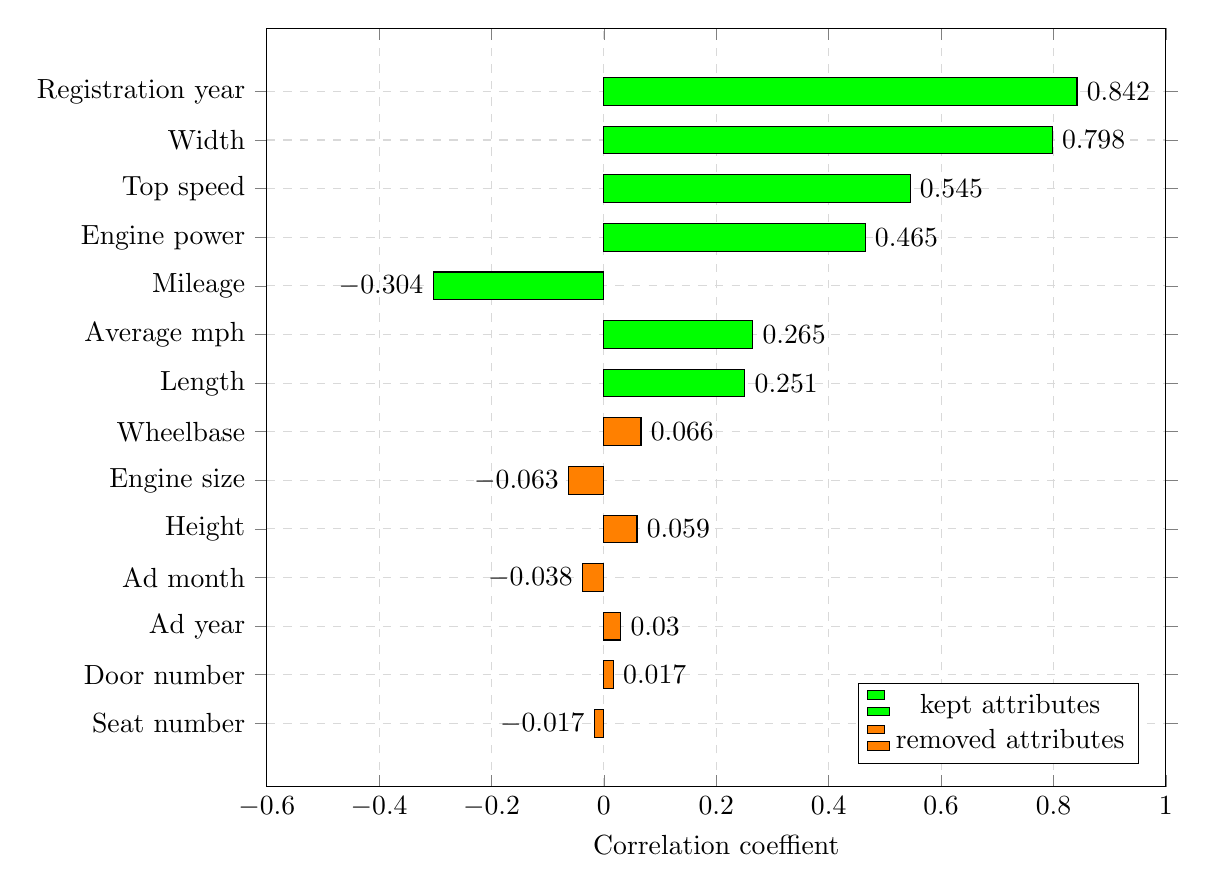
\begin{tikzpicture}
        \begin{axis}[
            xbar,
            xmin=-0.6,
            xmax=1,
            xtick={-0.6, -0.4, -0.2, 0, 0.2, 0.4, 0.6, 0.8, 1},
            legend pos=south east,
            grid=major, grid style={dashed,gray!30},
            width=13cm,
            xlabel={Correlation coeffient},
            symbolic y coords={Seat number,Door number,Ad year,Ad month,Height,Engine size,Wheelbase,Length,Average mph,Mileage,Engine power,Top speed,Width,Registration year},
            ytick={Seat number,Door number,Ad year,Ad month,Height,Engine size,Wheelbase,Length,Average mph,Mileage,Engine power,Top speed,Width,Registration year},
            nodes near coords,
            nodes near coords align={horizontal},
            every node near coord/.style={/pgf/number format/fixed, /pgf/number format/precision=3},
            /pgf/bar shift={0pt},
            ]
            \addplot [fill=green] coordinates {
                (0.251,Length)
                (0.265,Average mph)
                (-0.304,Mileage)
                (0.465,Engine power)
                (0.545,Top speed)
                (0.798,Width)
                (0.842,Registration year)
                };
            \addplot [fill=orange] coordinates {
                (-0.017,Seat number)
                (0.017,Door number)
                (0.03,Ad year)
                (-0.038,Ad month)
                (0.059,Height)
                (-0.063,Engine size)
                (0.066,Wheelbase)
                };
            \legend{kept attributes, removed attributes}
        \end{axis}
    \end{tikzpicture}
    \caption{Correlation with the price attribute}
    \label{fig:correlationdiagram}
\end{figure}

\autoref{fig:correlationdiagram} shows the results which include both positive and negative correlation. Positive correlation means that if the value of attribute 1
increases, the value of attribute 2 does as well. A logical example is the engine power, as it makes sense that a more powerful car sells for a higher price. On the other hand
negative correlation describes the opposite. A higher mileage results in a lower price as it indicates higher wear.
\par
In the figure the attributes are listed from the highest to the least influence on the price. As the ones marked in color orange do not really have an affect, they are removed from
the data set and only those highlighted in green are kept.

\subsubsection{Removing attributes and setting target}
In the next step not only the attributes with low correlation, but also the non-numeric ones are removed. This is the case as they can't be used in the calculation
of the linear regression model without further preprocessing and because the model is good enough already without them. Additionally, the price is set as 
target value, which is required for the linear regression module in Orange.

\subsubsection{Dividing data set and Calculating Linear Regression}


\section{Linear Regression Model}
\subsection{Results}

\subsection{Visualization}
\begin{figure}[h]
    \begin{tikzpicture}
        \begin{axis}[
            clip mode=individual,
            legend pos=south east,
            xmin=400,
            xmax=20000,
            ymin=400,
            ymax=20000,
            xlabel={Actual price \lbrack\pounds\rbrack},
            ylabel={Model's calculated price \lbrack\pounds\rbrack},
            xtick={2000, 6000, 10000, 14000, 18000},
            ytick={2000, 6000, 10000, 14000, 18000},
            width=13cm,
            scaled ticks=false,
            tick label style={/pgf/number format/fixed},
            y label style={yshift=1.2em}
            ]
        \addplot [mark=none,color=blue,style=very thick]
          table [y={create col/linear regression={y=model_price}}, col sep=comma] {./other/Linear_regression.csv};
          \addlegendentry{Regression line}  
          \addplot [mark=*,color=red,only marks]
          table [x=actual_price, y=model_price, col sep=comma] {./other/Linear_regression.csv};
                 
        \end{axis}
      \end{tikzpicture}
    \caption{Plotted Linear Regression Model}
    \label{fig:linearregressiondiagram}
\end{figure}